\def\L{\textless}
\def\G{\textgreater}
\chapter{METHODOLOGY}

In this chapter, we examine the methods used in our analysis in detail to answer the research questions \emph{\textbf{R1}} to \emph{\textbf{R4}}. We begin with the background of the Stackoverflow questions and answers. Next, our methodology to perform sentiment analysis. Finally, we discuss the methods to find whether correlations exist within the datasets.

\section{Stackoverflow Questions and Answers}
It is essential to understand the structure of Stackoverflow questions and answers and their usage in our analysis. When a registered Stackoverflow participant posts a question related to software topics, the post generates question metadata. Similarly, when a participant answers the posted question, it generates answer metadata. When the participant requesting the question receives a relevant answer, the most relevant answer becomes an accepted answer. The Stackoverflow participant and platform are the two sources that generate the question metadata. The participant generates the question title, descriptive question body, relevant tags, and accepted answer. While the Stackoverflow platform generates the unique identifier, date and time of the post, the number of favorites, score, and the number of views to the question. 

Similarly, the answer metadata has two sources, where the participant generates the answer body, and the platform generates the answer identifier and date. When participants post duplicate questions, the Stackoverflow platform often merges the two questions into one. If a participant considers and marks an answer as a relevant solution for this problem, then the Stackoverflow platform considers that answer as an accepted answer. For an example question and answer metadata, refer to the Table \ref{questions} and the Table \ref{answers} and note the metadata updates with time.

\begin{table}[t!hb]
\caption{Stackoverflow Sample Question}
\label{questions}
% this question has neutral sentiment: positive
\centering
\begin{tabular}{p{1.7in}p{1.5in}p{2.5in}} \hline
\textbf{Question Metadata} & \textbf{Description} & \textbf{Example}\\ \hline
question id & unique identifier & 47613802\\ 
\\
title & title given by user & how to create threads dynamically? \\
\\
body & question content & I want to create certain number of threads in my program where the number of threads to be created is provided by the user at run-time\\
\\
date & time and date of post & 2017-12-02 23:44:13.160\\ 
\\
tags & Stackoverflow tags & multithreading, java, dynamic\\
\\
favorites & count of user likes & 79\\ 
\\
score & like and dislike score & 150\\
\\
views & total views & 454\\
\\
accepted answer & user accepted answer & 47613819 \\ \hline
\end{tabular}
\end{table}


\begin{table}[b!ht]
\caption{Stackoverflow Sample Answer}
\label{answers}
\centering
\begin{tabular}{p{1.7in}p{1.5in}p{2.5in}} \hline
\textbf{Answer Metadata} & \textbf{Description} & \textbf{Example}\\\hline
answer id & a unique identifier & 47613819 \\ 
\\
date & time and date of post & 2017-12-02 23:47:28.157 \\
\\
body & an answer to question & there are a number of ways to do this. A for loop is the easiest your runnable couple be something like this\\ \hline
\end{tabular}
\end{table}


\section{Concurrency and Big Data Datasets}

To perform our sentiment analysis study, we begin by examining the data for concur- rency \cite{ahmed2018concurrency} and big data \cite{bagherzadeh2019going} by using the two datasets from the previous publications. These two papers analyze the Stackoverflow question and answer posts from the Stackoverflow official data dump, which is publicly available at \cite{stackoverflow2019}. In this section, we discuss the contents of the two datasets, as shown in Figure \ref{last}; these are the questions and answers, the topics, and the measures for popularity and difficulty metrics.

\subsection{Concurrency and Big Data Questions and Answers}
\label{dataset}
For concurrency dataset, we utilized Ahmed and Bagherzadeh's work \cite{ahmed2018concurrency}, which analyzes the Stackoverflow data over 9 years from August 2008 until December 2017. This dataset includes 38,485,046 questions and answers posted by 3,589,412 software developer participants of the Stackoverflow platform. Among these posts, 14,995,834 (39\%) are questions and 23,489,212 (61\%) are answers. From 38,485,046 questions and answers, the study concluded by identifying 245,576 (64\%) of questions and answers belonging to the topic of concurrency. In those concurrency posts of the total of 245,576 questions and answers, 156,812 (64\%) belong to question posts and 88,764 (36\%) belonging to answer posts.

To study big data developers, we utilized the data from Bagherzadeh and Khatchad- ourian \cite{bagherzadeh2019going} work, which categorizes Stackoverflow questions and answers as big data topics. The input dataset for the study includes 42,850,541 Stackoverflow questions and answers posted by 4,142,516 software developers over a 10-year duration from August 2008 to December 2018. The study identifying 157,525 questions and answers belonging to big data topics of those, 112,948 (72\%) are questions, and 44,577 (28\%) are answers. Our study aggregates both papers, and our dataset input has 403,413 questions and answers containing 269,818 (67\%) questions and 133,595 (33\%) answers. To see the statistics of our dataset, refer to Table \ref{tabStat}. We perform sentiment analysis on 403,413 questions and answers to answer our research questions.

\subsection{Concurrency and Big Data Topics} 
\label{topicssec}
To study the sentiment of concurrency and big data topics, we utilize the topic categorization conducted by the papers \cite{ahmed2018concurrency, bagherzadeh2019going}. These two works categorize the questions and answers using Latent Dirichlet Allocation (LDA) \cite{blei2003latent} and an open card sort. Topic modeling using LDA means assigning related topic names over a normal distribution based on keywords existing in the question and answer. And, an open card sort means that topic names are not predefined but assigned in the topic labeling process. The topic labeling process the studies \cite{ahmed2018concurrency, bagherzadeh2019going} follow, is that they manually sample through 15 random posts from individual topics. By iteratively refining associated topics, 27 topics names were manually assigned to 245,576 concurrency questions and answers. To see the concurrency topic names and their descriptions, refer to Table \ref{tab:CT}. For 157,525 big data questions and answers, the study \cite{bagherzadeh2019going} assigns them to 28 big data topics. For detailed big data topic names and descriptions, refer to Table \ref{tab:BT}. We perform sentiment analysis to assess sentiments for each topic in concurrency and big data datasets.

\begin{table}[h!bt]
\caption{Statistics of Concurrency and Big Data Dataset}
\label{tabStat}
\centering 
\begin{tabular}{p{.9in}p{1.4in}p{1.4in}p{1.4in}} \hline
\textbf{Dataset} & \textbf{No. of Q\&As} & \textbf{No. of Questions} & \textbf{No. of Answers}\\  \hline
concurrency & 245,576 & 156,812 (64\%) & 88,764 (36\%) \\
\\
big data & 157,525 & 112,948 (72\%) & 44,577 (28\%) \\\hline
\textbf{Total} & \textbf{403,413} & \textbf{269,818 (67\%)} & \textbf{133,595 (33\%)} \\ \hline
\end{tabular}
\end{table}

\begin{table}[tbp]
\caption{Concurrency Topics From the Previous Work \cite{ahmed2018concurrency}}
\centering
\label{tab:CT}
\begin{tabular}{p{.15in}p{2.25in}p{3.1in}}\hline
%\textbf{No.}&\textbf{Topic}&\textbf{Topic Description for Q \& A's }\\ \hline
\textbf{No.}&\textbf{Topic}&\textbf{Q \& As Topic Words}\\ \hline
1&basic concepts & 
code understand read find edit make\\

2&task parallelism & 
task schedul async asynchron parallel\\

3&producer-consumer concurrency & 
queue consum produc process buffer block\\

4&parallel computing & 
parallel node loop comput openmp mpi\\

5&process life cycle management& 
process child parent termin fork kill start\\

6&python multiprocessing& 
python script run multiprocess parallel php\\

7&thread life cycle management& 
thread execut background separ join finish\\

8&thread sharing& 
variabl pass call pointer pthread global\\

9&thread scheduling& 
loop time wait stop run start sleep set check\\

10&thread pool & 
pool job process task limit threadpool\\

11&concurrent collections& 
list arrai map element collect iter kei add\\

12&thread safety& 
thread java safe multipl multi multithread\\

13&locking& 
lock mutex wait condit semaphor acquir\\

14&memory consistency& 
read write variabl atom cach share synchron\\

15&entity management& 
concurr session spring entiti transact actor\\

16&database management systems& 
databas tabl queri row record lock insert sql\\

17&file management& 
file read write log line open stream directori\\

18&object-oriented concurrency& 
object class method creat static access\\

19&web concurrency& 
servic web server applic user app net http\\

20&event-based concurrency& 
event signal handler timer callback call slot\\

21&mobile concurrency& 
android app view updat frame asynctask\\

22&client-server concurrency& 
connect send socket receiv port read\\

23&data scraping& 
data time load download problem\\

24&runtime speedup& 
cpu core time performance\\

25&unexpected output& 
code work run output problem print line\\

26&irreproducible behavior& 
error run problem applic compil crash\\

27&GUI& 
updating gui windows applications\\ \hline
\end{tabular}
\end{table}

\begin{table}[tbp]
\caption{Big Data Topics From the Previous Work \cite{bagherzadeh2019going}}
\centering
\label{tab:BT}
\begin{tabular}{p{.15in}p{2.25in}p{3.1in}}\hline
\textbf{No.}&\textbf{Topic}&\textbf{Q \& As Topic Words}\\ \hline
1&memory management & 
memori executor task job spark run core\\ 

2&PIG& 
pig scripts oozi job workflow action run error\\ 

3&connection& 
connect hadoop server instal cloudera\\ 

4&dataset load\&store & 
file data spark read json csv parquet load\\ 

5&data organization& 
partit join data number case oper kei set\\ 

6&scala spark& 
scala spark org apach java sql appli anonfun\\ 

7&pyspark& 
python pyspark spark zeppelin error run\\ 

8&dataframe& 
column datafram row spark pyspark data\\ 

9&file distribution& 
node hadoop cluster namenod hdf datanod\\

10&general programming& 
class function method object call code type\\ 

11&debugging& 
error code run work problem issu except fail\\ 

12&hbase& 
hbase tabl row region zookeep client scan\\ 

13&job management& 
spark run cluster job applic submit yarn\\ 

14&file format& 
file line read input split text block size data\\

15&file management& 
file hdf directori path hadoop folder local\\ 

16&string& 
string type field arrai null column valu\\ 

17&database import\&export& 
sqoop cassandra jdbc mysql databas connector\\ 

18&stream processing& 
stream spark kafka data messag batch process\\ 

19&basic concepts& 
data hadoop process system databas solut\\ 

20&date\&time& 
date time timestamp data month event record\\ 

21&logging& 
info flume log java org channel apach sink\\ 

22&performance& 
data perform memori process size run million\\ 

23&text search& 
document mongodb queri collect elastic search\\ 

24&dependency management& 
jar hadoop version spark java error run depend\\ 

25&debugging& 
java org apach hadoop lang run mapr util\\ 

26&machine learning& 
model spark vector mahout train featur data\\ 

27&hive analysis& 
hive tabl queri creat data sql select insert\\ 

28&mapreduce& 
kei group count reduc hadoop map reduc\\ 

29&RDD& 
rdd spark transform code function scala map\\ \hline
\end{tabular}
\end{table}

\clearpage
\subsection{Concurrency and Big Data Popularity and Difficulty}
We utilized popularity and difficulty metrics for the concurrency and big data topics from \cite{ahmed2018concurrency, bagherzadeh2019going} to determine the correlation between sentiment with popularity and sentiment with difficulty. The authors evaluated popularity and difficulty metrics using questions and answers metadata of the Stackoverflow, given in Table \ref{questions} and the Table \ref{answers}. The popularity metric was calculated by 3 well-known measures, which are the average views, average favorites, and average scores. Likewise, they evaluated the difficulty metric using 2 well-known measures, which are the percentage of questions without accepted answers and the hours to receive an accepted answer.

To be more specific, the definitions of the popularity metrics are as follows; they defined average views measure \cite{bajaj2014mining, nadi2016jumping, rosen2016mobile, yang2016security} as the average number of visits to the posted question to the number of questions in a topic. They considered the average views measure because Stackoverflow allows both registered and unregistered users to visit questions. We consider average views because the number of views to the Stackoverflow platform by the unregistered users is higher in number compared to registered users \cite{mamykina2011design}. Secondly, as defined in \cite{bajaj2014mining, nadi2016jumping, pinto2015study, yang2016security}, the average favorites measure uses the question metadata’s favorites counter by taking the average of it within a topic. To be more specific, the average favorites is the total number of registered users who mark the question as to their favorites. Finally, as defined in \cite{bajaj2014mining, nadi2016jumping, pinto2015study, yang2016security}, the average scores measure is calculating the average of the question metadata’s scores counter within a topic. To be more specific, the average scores is the total number of registered users who like or dislike the question. For more details about popularity metrics, refer to Table \ref{PM}.

\begin{table}[h!tb]
\caption{Popularity and Difficulty Metrics}
\label{PM}
\centering
\begin{tabular}{p{0.70in}p{1.20in}p{3.60in}} \hline
\textbf{Metrics} & \textbf{Measures} & \textbf{Description}\\ \hline
popularity & average views & an average number of views for all the questions in a topic the questions in a topic \\
\\
& average favorites & total average of users marking the question as their as their favorite in a topic \\
\\
& average scores & average of raw score for all the questions within a topic \\
\\
difficulty & \%w/o acc. answer & percentage of questions without accepted answers \\
\\
& hrs to acc. answer & average median time needed for questions of a topic to receive accepted answers\\ \hline
\end{tabular}
\end{table}

On the other hand, the difficulty metric defined 2 measures that are as follows. The first measure the percentage of questions that do not have accepted answers within a topic \cite{rosen2016mobile, treude2011programmers,yang2016security}. The second measure checks the average time that is taken for a question in a topic to receive an accepted answer \cite{rosen2016mobile, yang2016security}. More straightforward questions tend to receive solutions faster compared to harder questions. Measures of the difficulty metric are in Table \ref{PM}.

The authors in \cite{ahmed2018concurrency, bagherzadeh2019going} calculated popularity and difficulty metrics for concurrency and big data topics using the five measures defined as above. Note, the values calculated for the measures dependent on questions and answers metadata and the time the information is gathered. The values for the popularity and difficulty measures for the concurrency topics are in the Table \ref{CP}. Likewise, the values for these two measures for the big data topics are in Table \ref{BP}.

\begin{table}[tbp]
\caption{Popularity and Difficulty Metrics for the Concurrency Topics From the Previous Work \cite{ahmed2018concurrency}}
\label{CP}
%\begin{tabular}{p{1.5in}p{.6in}p{.6in}p{.6in}p{.7in}p{.6in}} \hline
\begin{tabular}{p{1.7in}p{.5in}p{.6in}p{.4in}p{.9in}p{.9in}} \\ \hline
\textbf{Topic} & \textbf{Popularity} & & & \textbf{Difficulty} \\\hline
& \textbf{Avg. views} & \textbf{Avg. favorites} & \textbf{Avg. scores} & \textbf{\%w/o acc. answer} & \textbf{Hrs to acc. answer}\\ \hline
thread safety & 2848 & 1.5 & 4.6 & 39.6 & 0. 3\\ 
basic concepts & 2222 & 1.6 & 4.3 & 37.0 & 0.7 \\ 
task parallelism & 2216 & 1.3 & 4.0 & 35.3 & 0.4 \\ 
locking & 2152 & 1.3 & 3.5 & 40.1 & 0.3\\ 
thread life cycle management & 2130 & 0.7 & 2.4 & 40.4 & 0.3\\ 
thread scheduling & 2032 & 0.7 & 2.2 & 40.8 & 0.4\\ 
process life cycle management & 2004 & 1.0 & 2.6 & 44.9 & 0.6\\ 
thread pool & 1841 & 0.9 & 2.7 & 47.0 & 0.7\\ 
object-oriented concurrency & 1773 & 0.8 & 2.6 & 35.2 & 0.3\\ 
database management systems & 1727 & 0.6 & 1.8 & 51.2 & 1.0\\ 
thread sharing & 1671 & 0.6 & 2.0 & 35.6 & 0.3\\ 
GUI & 1664 & 0.5 & 1.6 & 41.1 & 0.4\\ 
irreproducible behavior & 1647 & 0.6 & 2.3 & 51.1 & 2.1\\ 
event-based concurrency & 1636 & 0.7 & 2.3 & 39.7 & 0.6 \\ 
python multiprocessing & 1587 & 0.9 & 2.5 & 50.3 & 0.9 \\ 
entity management & 1583 & 0.8 & 2.3 & 48.0 & 1.8\\ 
memory consistency & 1531 & 1.7 & 4.8 & 33.2 & 0.4\\ 
file management & 1458 & 0.6 & 1.9 & 48.8 & 0.6\\ 
producer-consumer concurrency & 1311 & 0.8 & 2.2 & 43.3 & 0.7\\ 
unexpected output & 1304 & 0.5 & 1.6 & 41.8 & 0.7\\ 
mobile concurrency & 1292 & 0.5 & 1.3 & 50.4 & 0.8\\ 
runtime speedup & 1276 & 0.9 & 2.7 & 48.0 & 0.7\\ 
web concurrency & 1252 & 0.8 & 1.9 & 50.7 & 0.9 \\ 
concurrent collections & 1155 & 0.5 & 2.0 & 38.6 & 0.4 \\ 
client-server concurrency & 1083 & 0.4 & 1.1 & 50.4 & 0.9\\ 
data scraping & 1003 & 0.6 & 1.4 & 48.9 & 1.0 \\ 
parallel computing & 899 & 0.6 & 1.9 & 50.1 & 2.1\\ \hline
\textbf{Average} & \textbf{1640.6} & \textbf{0.8} & \textbf{2.4} & \textbf{43.7} & \textbf{0.7}\\ \hline
\end{tabular}
\end{table}

\begin{table}[tbp]
\caption{Popularity and Difficulty Metrics for the Big Data Topics From the Previous Work \cite{bagherzadeh2019going}}
\label{BP}
\centering
\begin{tabular}{p{1.4in}p{.5in}p{.6in}p{.4in}p{.9in}p{.9in}} \hline
% \begin{tabular}{p{1.8in}p{.4in}p{.6in}p{.4in}p{.9in}p{.9in}} \hline
\textbf{Topic} & \textbf{Popularity} & & & \textbf{Difficulty} \\ \hline
& \textbf{Avg. views} & \textbf{Avg. favorites} & \textbf{Avg. scores} & \textbf{\%w/o acc. answer} & \textbf{Hrs to acc. answer}\\ \hline
file management & 2141.6 & 0.5 & 1.4 & 62.3 & 3.7 \\
file distribution & 1861.6 & 0.5 & 1.3 & 63.1 & 6.7 \\
hive & 1811.6 & 0.3 & 1.0 & 66.0 & 3.6\\
dependency management & 1774.7 & 0.4 & 1.4 & 64.2 & 4.7\\
dataframe & 1731.4 & 0.5 & 1.3 & 46.3 & 1.2 \\
string & 1600.8 & 0.3 & 1.0 & 51.9 & 1.3\\
RDD & 1543.8 & 0.5 & 1.6 & 49.4 & 1.1\\
hbase & 1464.9 & 0.4 & 1.3 & 63.4 & 17.2 \\
dataset load\&store & 1410.7 & 0.4 & 1.2 & 63.5 & 2.9\\
data organization & 1369.3 & 0.8 & 2.0 & 58.5 & 3.2\\
file format & 1315.1 & 0.5 & 1.2 & 61.9 & 4.0\\
connection management & 1301.7 & 0.3 & 1.0 & 68.7 & 17.0\\
mapreduce model & 1294.2 & 0.5 & 1.2 & 51.6 & 0.2\\
debugging & 1278.3 & 0.3 & 1.2 & 64.3 & 2.4\\
basic concepts & 1248.7 & 0.9 & 1.8 & 59.8 & 5.5\\
pyspark & 1152.5 & 0.4 & 1.3 & 68.1 & 7.6 \\
memory management & 1141.1 & 0.6 & 1.7 & 69.0 & 7.7 \\
job management & 1131.2 & 0.4 & 1.5 & 65.7 & 9.2 \\
general programming & 1130.9 & 0.5 & 1.6 & 53.8 & 1.8\\
PIG & 1079.8 & 0.2 & 0.8 & 63.0 & 10.1 \\
date\&time & 1068.1 & 0.3 & 0.7 & 55.8 & 2.1 \\
text search & 1053.8 & 0.5 & 1.3 & 57.5 & 5.2\\
scala spark & 1050.0 & 0.3 & 1.0 & 64.8 & 2.6\\
database import\&export & 1048.7 & 0.3 & 0.8 & 69.8 & 7.9 \\
performance & 840.3 & 0.5 & 1.4 & 64.0 & 3.8\\
logging & 820.7 & 0.3 & 0.8 & 66.9 & 22.5 \\
machine learning & 763.9 & 0.5 & 1.3 & 61.6 & 4.6\\
stream processing & 715.0 & 0.4 & 1.2 & 71.3 & 7.4\\ \hline
\textbf{Average} & \textbf{1290.8} & \textbf{0.4} & \textbf{1.2} & \textbf{61.6} & \textbf{5.9} \\ \hline
\end{tabular}
\end{table}

\section{Sentiment Analysis}

To perform our sentiment analysis, we followed the following steps: For Step 1, we removed noise by preprocessing the Stackoverflow question and answers. In Step 2, we analyzed the sentiment of Stackoverflow questions and answers by using the tool Senti4SD for concurrency and big data datasets. In Step 3, we measured the sentiment for topics in the concurrency and the big data topics, which are in the Tables \ref{tab:CT} and the Table \ref{tab:BT}, respectively. In the final step, we calculated correlations between sentiment with popularity and sentiment with difficulty using Kendall Tau bivariant correlation. 

\subsection{Preprocessing}
Determining the sentiment of text with noise could lead to incorrect results. So, the text should be free of hidden metadata to perform the sentiment analysis. Consequently, we preprocessed the body of the questions and the body of the answer to reduce noise. A more thorough explanation for the preprocessing is getting a plain text, which we define as a piece of text containing alphanumeric characters.

We start by removing the code snippets that contain code using natural language processing. That is, we removed the tags {\L/code\G} and {\L/code\G} from the questions and answers metadata. Then, we remove all remaining HTML tags such as paragraph tags {\L/p\G} and {\L/p\G}, URL tags {\L/a\G} and {\L/a\G} and nbsp; extra spaces tag. 

\begin{table}[b!ht]
\caption{Preprocessing Example}
\label{tab:example}
\centering
% {|lll|}SSS
\begin{tabular} {p{3in}p{2.5in}}\hline
\textbf{Input Text} & \textbf{Processed Text} \\ \hline

body: \&lt;p\&gt; i use retrofit to get the response correctly, then i pass the response to an object in the response body, while it fails to get the object in, ui thread there is a nullpointerexception, error i think it's the problem of the asynchronous request, how can i avoid this problem? \&lt;p\&gt;?\&lt;/p\&gt; \&\#xA;\&\#xA;\&lt;pre\&gt;\&lt;code\&gt; \emph{multiple lines of code in java} \&\#xA;\&lt;/code\&gt;\&lt;/pre\&gt;\&\#xA;
&
i use retrofit to get the response correctly then i pass the response to an object in the response body while it fails to get the object in ui thread there is a nullpointerexception error i think it's the problem of asynchronous request how can i avoid this problem \emph{(removed)} \\ \hline
\end{tabular}
\end{table}

Furthermore, we removed any remaining newlines, extra spaces, and non-alphanum- eric characters using the Java library JSoup to parse the text and convert it to a plain text.

We preprocessed 400K Stackoverflow questions and answers to plain text that belong to both concurrency and big data datasets. For instance, a question's metadata before and after preprocessing can be seen in Table \ref{tab:example}. Here, the text in the left column represents the text before preprocessing, and the text in the right column gives the processed version of the same text.

\subsection{Senti4SD}

We utilize the tool Senti4SD to assess the sentiment, which can be either positive, negative, or neutral for the 400K Stackoverflow questions and answers belonging to both concurrency and big data datasets. For more details about the tool, Senti4SD refer \cite{calefato2018sentiment}. 

As discussed in section \ref{dataset}, the 400K Stackoverflow questions and answers are an aggregate of 250K concurrency dataset and 150K big data dataset. The sentiment analysis on this dataset performed, as shown in Figure \ref{step1}. A sample of Stackoverflow question processed by the Senti4SD tool is shown in the Table \ref{SE}, where the input is a preprocessed text as seen in the left column, and the output sentiment assessment for this text is in the right column.


\begin{table}[h!tb]
\caption{A Sample Stackoverflow Question and Its Sentiment}
\label{SE}
\centering
\begin{tabular}{p{3.5in}p{2in}}\hline
\textbf{Processed Text} & \textbf{Sentiment of Text} \\\hline
{i use retrofit to get the response correctly then i pass the response to an object in the response body while it fails to get the object in ui thread there is a nullpointerexception error i think it's the problem of the asynchronous request how can i avoid this problem} & {positive} \\ \hline 
\end{tabular}
\end{table}

\begin{figure}[h!tb]
\centering 
\includegraphics{Images/Sentiment}
\caption{Sentiment Analysis Using Senti4SD}
\label{step1}
\end{figure}

\subsection{Concurrency and Big Data Topics Sentiment}
\label{topicsenti}
In the previous section, we discussed the sentiment analysis tool Senti4SD to assess the sentiment of questions and answers belonging to concurrency and big data datasets. As the goal of our thesis is to answer the research questions \emph{\textbf{R1}} to \emph{\textbf{R4}}, we do so by understanding the relationship between a software developer's sentiment concerning popular and difficult concurrency and big data topics. We calculate the topic sentiment by taking the mean of the sentiment assessments (positive, negative, neutral) for all the Stackoverflow questions and answers within a topic.

\subsection{Correlations in Concurrency and Big Data}
\label{correlations}
To find the correlations within the concurrency and big data datasets, first, we gathered the results from our previous step of finding sentiment for each topic within these datasets. Next, we used the popularity and difficulty metrics calculated by the authors in \cite{ahmed2018concurrency, bagherzadeh2019going}. In total, our research finds correlations between three measures of sentiment with three measures of popularity metric and three measures of sentiment with two measures of difficulty metric. 

We find the correlations existing within concurrency and big data datasets using a rank-based correlation. For this, we use Kendall tau bivariant correlation, which in comparison to other rank-based correlations, is less sensitive to outliers, giving us relatively many stable results. Kendal tau computes the coefficient between two non-parametric variables belonging to the same set with different ranks. To test our hypothesis of statistical dependencies, we input our numerical results to the tool IBM SPSS \cite{IBM2019}. A non-parametric test means that the distribution is without any underlying assumptions. In short, it means that the distribution has no prior knowledge about the probabilities of the variables being assessed.

By evaluating the correlations given by the tool, we answer our research questions \emph{\textbf{R1}} to \emph{\textbf{R4}}. The flow of our analysis is in Figure \ref{last}. In the next chapter, we discuss our results in depth.

\begin{figure}[h!tb]
\centering
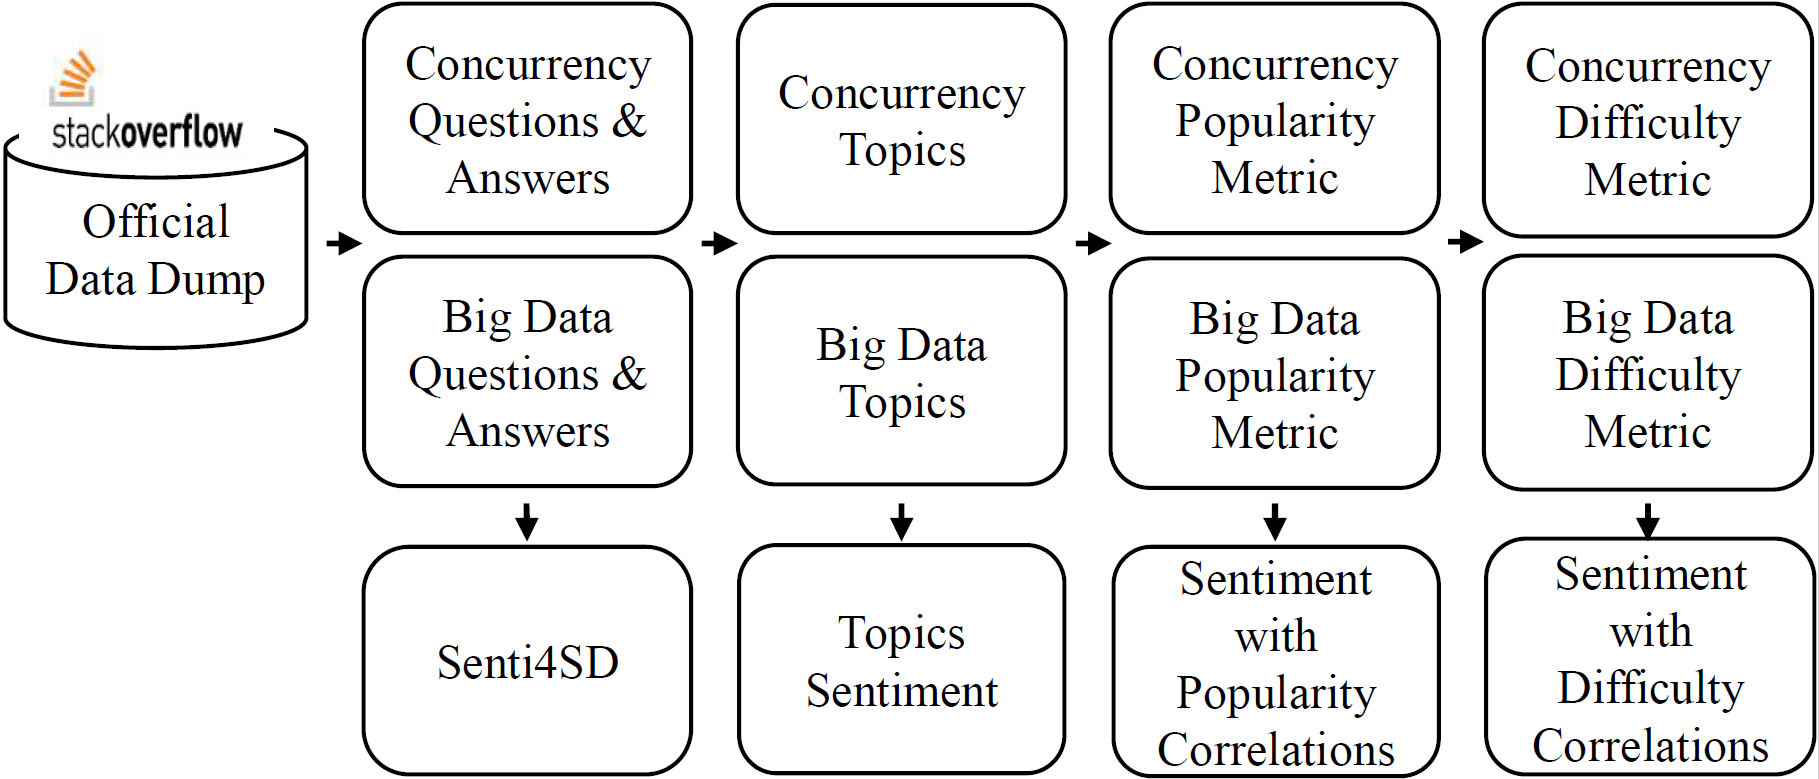
\includegraphics{Images/methodology}
\caption{Methodology}
\label{last}
\end{figure}